\subsection{Reasoning transfer in CLEVR-CoGenT}
\label{sec:reasoning-clevr}

\begin{figure}[htbp]
	\centering
	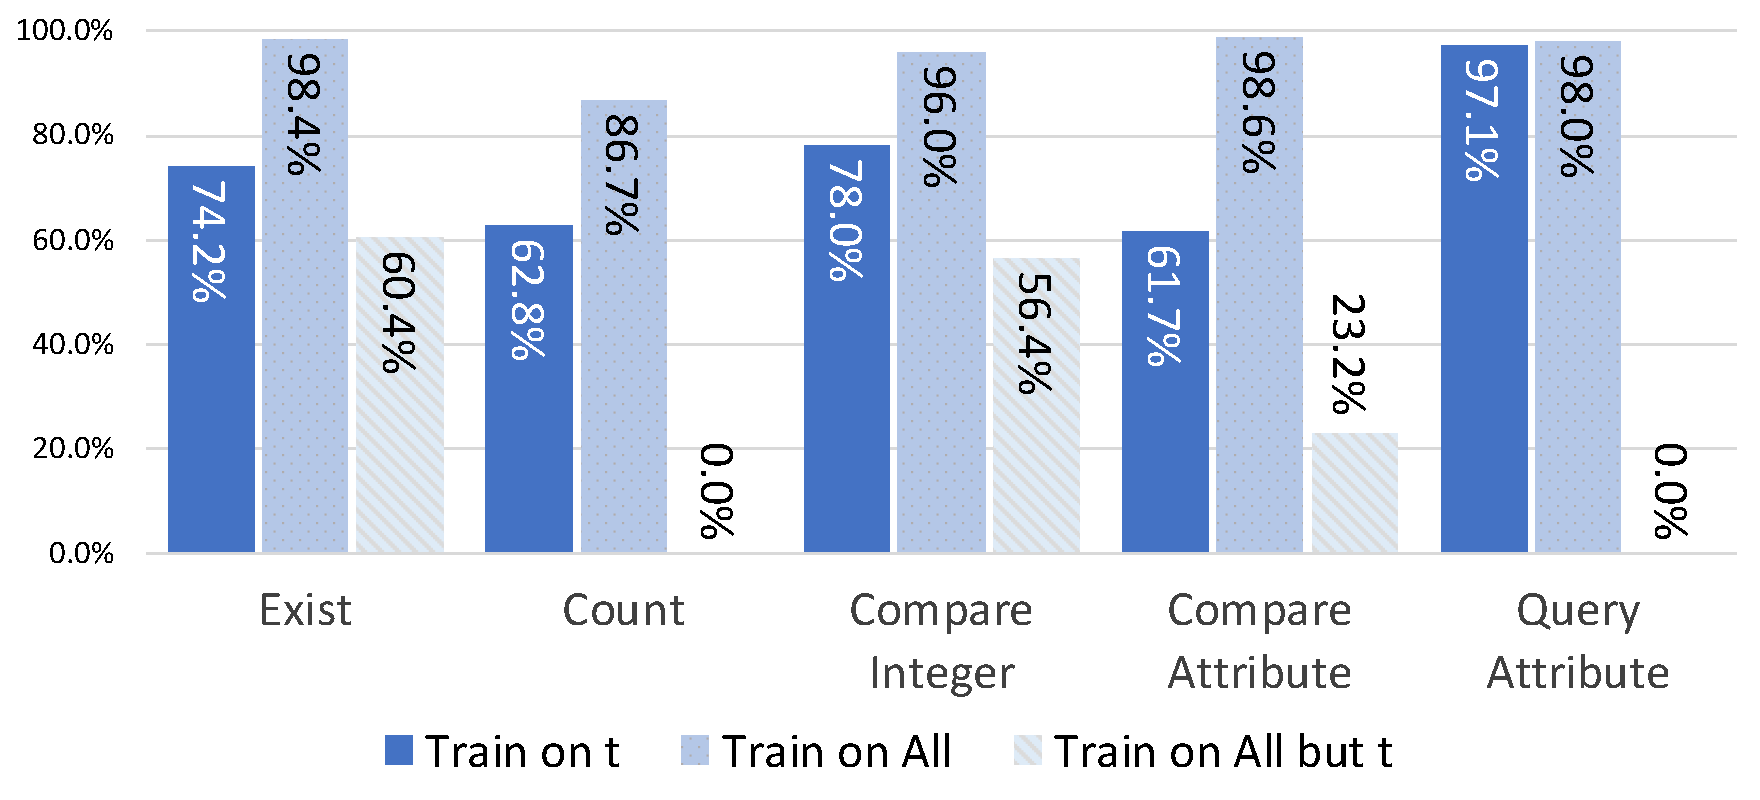
\includegraphics[width=\columnwidth]{../img/plots/cogent_reasoning_transfer.pdf}
	\caption{CoGenT-A accuracies for all tasks $t$ when training on $t$ only, training on all tasks jointly and training on all tasks but $t$.}
	\label{fig:CoGenT-results}
\end{figure}

Using the question categories defined by the author, we conduct the following experiments:
\begin{itemize}
	\compresslist
	\item Train and test SAMNet on a single task group $t$. These 5 experiments fit into the traditional ML setup of single-task learning;
	\item Train SAMNet on all task groups jointly and evaluate its performance on each task group $t$ separately.
	This is a transfer learning setting where for the source task family, the task is sampled from all questions, while for the target task family, the samples consist of questions from group $t$ only;
	\item Finally, for each task group $t$, we train SAMNet on all tasks but $t$, and test its performance on $t$. This can also be viewed as a transfer learning setting similar to the previous case.
\end{itemize}

Noticeable results are shown in~\cref{fig:CoGenT-results}, while the complete set is available in the supplementary material.

Looking at~\cref{fig:CoGenT-results}, SAMNet does well on \textit{Count} and \textit{QueryAttribute}, but poorer on the 3 other tasks in the single-task learning setting (blue). Indeed, \textit{Exist}, \textit{CompareInteger} and \textit{CompareAttribute} are binary tasks; \textit{Count} has output labels digits 0 through 10 (so $<$10\% accuracy by chance) and \textit{QueryAttribute} maps to the set of object-attribute values (15 labels).

Nevertheless, significant accuracy gains are noted when training jointly on all tasks (gray), ranging from 18 points to 37 points on 4 out of 5 tasks. These improvements suggest that related tasks benefit from joint training. \textit{QueryAttribute} only sees an increase of one point. One could qualify it as \textit{self-sufficient} as it does not appear to benefit from joint training with other tasks.

Finally, the ``all-tasks-but-$t$'' experiments (yellow) demonstrate that while tasks are related, one does not subsume another in terms of learning. Indeed, we can observe that for \textit{CompareAttribute}, while \textit{Exist} and \textit{CompareInteger} share the same output space, including them and holding out \textit{CompareAttribute} from the training set results in poor accuracy.
We also observe no learning for \textit{Count} and \textit{QueryAttribute}. As these categories have labels that do not overlap with other categories, the model cannot predict these labels.

An additional set of experiments, for which results are available in the supplementary material, fine-tune the model trained on all tasks on each task $t$ respectively.
Fine-tuning did not demonstrate a clear benefit (except for \textit{Count}, where the accuracy increased by 1.5 pt) without hurting performance on the other tasks. Nevertheless, these experiments leave open the possibility that joint training of tasks may potentially benefit from using weighted sampling towards the tail end with more emphasis on samples from less performing task groups, similar to~\cite{guo2018dynamic, kendall2018multi}.

\subsection{Reasoning transfer in COG}
\label{sec:reasoning-cog}

\begin{figure}[htbp]
	\centering
	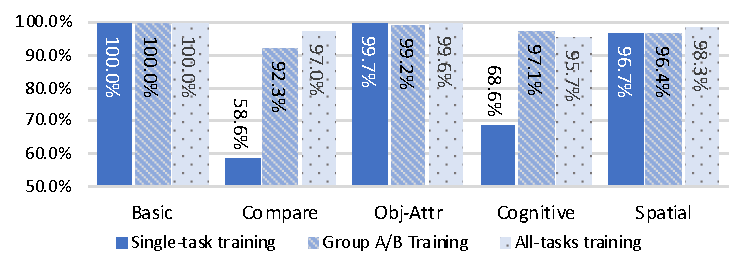
\includegraphics[width=\columnwidth]{../img/plots/cog_reasoning_transfer.pdf}
	\caption{COG accuracies for all task groups $t$ when training on $t$ only; training on Group A or B; and on all tasks.}
	\label{fig:COG-reasoning-results}
\end{figure}\vspace{2pt}

Reusing the task hierarchy in \cref{fig:task-groups}, we conduct the following experiments using the Canonical variant of COG to study whether transfer learning was effective in leveraging information gained by training a task family at a higher level
of the hierarchy:
 \begin{itemize}
 	\compresslist
	\item Train and test SAMNet on each of the 5 task groups at the lowest level of the hierarchy (Single-task training);
	\item Jointly train on:
	\begin{itemize}
		\item \textbf{Group A} and test on each task from the lowest groups (i.e. \textbf{Basic}, \textbf{Obj-Attr} and \textbf{Compare}) separately;
		\item \textbf{Group B} and test separately on \textbf{Spatial} and \textbf{Cognitive};
	\end{itemize}
	\item As a baseline, we compared the above results to the earlier experiment shown in~\cref{fig:samnet_cog_detailed}, which can be viewed as training jointly on \textbf{All} and testing on each group at the leaf level separately (All-task training).
\end{itemize}

The results of these experiments are shown in~\cref{fig:COG-reasoning-results}.

First, notice that for each of the \textbf{Basic} and \textbf{Obj-Attr} task families, the accuracy is near-perfect in all cases, suggesting that each contains the most primitive tasks and therefore do not benefit from training with other task families.
With \textbf{Spatial}, we see a small improvement showing that there is some benefit due to joint training with other task families.
Two groups that demonstrated a huge improvement of more than 25 points are \textbf{Compare} and \textbf{Cognitive}.
The former saw an accuracy jump from 58.6\% by training on samples from that family alone
to 97.0\% when training on all samples. To further emphasize this behavior, notice that
just joining \textbf{Compare} with \textbf{Obj-Attr} and \textbf{Basic} already causes a significant accuracy jump to 92.3\%.
In hindsight, this is not surprising, as the questions in \textbf{Compare} are composed
of fragments of questions given by \textbf{Basic} and \textbf{Obj-Attr}, and therefore can leverage the reasoning strategies developed there to reason about questions in \textbf{Compare}.
Lastly, for the \textbf{Spatial} family, we again see the benefits of joint training with all questions (68.6\% to 95.7\%) but in this case there
is a slight loss incurred by including everything. As seen in the figure, just jointly training with \textbf{Spatial} alone is sufficient to get a boost in accuracy (97.1\%). To summarize, while joint training helps, one needs to determine how much of correlation is present with the other tasks.
